% ĐỢT 5: CỤM 3 (ĐỀ 3) & CỤM 4 (ĐỀ 1) - BỘ ĐỀ THAM KHẢO TUYỂN SINH 10 NĂM HỌC 2026-2027 SỞ GD&ĐT TP.HCM

% ==============================================================================
% CỤM 3 - ĐỀ THAM KHẢO 3 (Trang 19-20, Đề số 9)
% ==============================================================================

\begin{bt}%[9D6H18-2]
% nguon: Đề tham khảo Tuyển sinh 10 năm học 2026-2027 Sở GD&ĐT TP.HCM - Cụm 3 Đề 3 - Bài 1
Cho hàm số $y = -\dfrac{1}{2}x^2$ có đồ thị là parabol $(P)$.
\begin{enumerate}[a)]
	\item Vẽ đồ thị $(P)$ trên mặt phẳng tọa độ $Oxy$.
	\item Tìm những điểm thuộc đồ thị $(P)$ có hoành độ gấp hai lần tung độ.
\end{enumerate}
\loigiai{
\begin{enumerate}[a)]
	\item Bảng giá trị của hàm số $y = -\dfrac{1}{2}x^2$:
	\begin{center}
		\begin{tabular}{|c|c|c|c|c|c|}
			\hline
			$x$ & $-4$ & $-2$ & $0$ & $2$ & $4$ \\ \hline
			$y$ & $-8$ & $-2$ & $0$ & $-2$ & $-8$ \\ \hline
		\end{tabular}
	\end{center}
	Đồ thị $(P)$ là một parabol đi qua các điểm $(-4; -8)$, $(-2; -2)$, $(0; 0)$, $(2; -2)$, $(4; -8)$, nhận trục tung $Oy$ làm trục đối xứng và có đỉnh là gốc tọa độ $O(0;0)$.
	\begin{center}
		\begin{tikzpicture}[>=stealth,scale=0.7]
			\draw[->] (-5,0) -- (5,0) node[below] {$x$};
			\draw[->] (0,-9) -- (0,1.5) node[left] {$y$};
			\draw (0,0) node[above right] {$O$};
			\foreach \x in {-4,-2,2,4}
				\draw (\x,0.1) -- (\x,-0.1) node[above] {\small $\x$};
			\foreach \y in {-8,-2}
				\draw (0.1,\y) -- (-0.1,\y) node[left] {\small $\y$};
			\draw[dashed] (-2,0) -- (-2,-2) -- (2,-2) -- (2,0);
			\draw[dashed] (-4,0) -- (-4,-8) -- (4,-8) -- (4,0);
			\draw[thick,smooth,samples=100,domain=-4.2:4.2] plot(\x,{-0.5*(\x)^2});
			\node[below right] at (2,-2) {$(P)$};
		\end{tikzpicture}
	\end{center}
	\item Gọi $M(x; y)$ là điểm thuộc đồ thị $(P)$ có hoành độ gấp hai lần tung độ.\\
	Ta có $x = 2y \implies y = \dfrac{1}{2}x$.\\
	Vì $M \in (P)$ nên ta có phương trình hoành độ giao điểm:
	$$\dfrac{1}{2}x = -\dfrac{1}{2}x^2 \iff \dfrac{1}{2}x^2 + \dfrac{1}{2}x = 0 \iff \dfrac{1}{2}x(x + 1) = 0 \iff \left[\begin{aligned} &x = 0 \\ &x = -1. \end{aligned}\right.$$
	\begin{itemize}
		\item Với $x = 0 \implies y = 0$, ta được điểm $O(0; 0)$.
		\item Với $x = -1 \implies y = -\dfrac{1}{2}$, ta được điểm $\left(-1; -\dfrac{1}{2}\right)$.
	\end{itemize}
	Vậy tọa độ các điểm cần tìm là $(0; 0)$ và $\left(-1; -\dfrac{1}{2}\right)$.
\end{enumerate}
}
\end{bt}

\begin{bt}%[9D6H20-2]
% nguon: Đề tham khảo Tuyển sinh 10 năm học 2026-2027 Sở GD&ĐT TP.HCM - Cụm 3 Đề 3 - Bài 2
Cho phương trình bậc hai $2x^2 - 7x + 4 = 0$.
\begin{enumerate}[a)]
	\item Chứng minh phương trình trên luôn có hai nghiệm phân biệt $x_1, x_2$.
	\item Không giải phương trình, hãy tính giá trị của biểu thức:
	$$Q = \dfrac{x_1}{x_2 + 2} - x_1 + \dfrac{x_2}{x_1 + 2} - x_2.$$
\end{enumerate}
\loigiai{
\begin{enumerate}[a)]
	\item Phương trình $2x^2 - 7x + 4 = 0$ có các hệ số $a = 2$, $b = -7$, $c = 4$.\\
	Biệt thức:
	$$\Delta = b^2 - 4ac = (-7)^2 - 4 \cdot 2 \cdot 4 = 49 - 32 = 17 > 0.$$
	Vì $\Delta > 0$ nên phương trình luôn có hai nghiệm phân biệt $x_1, x_2$.
	\item Theo định lí Vi-ét, ta có:
	$$\left\{\begin{aligned} &x_1 + x_2 = \dfrac{7}{2} \\ &x_1 x_2 = \dfrac{4}{2} = 2. \end{aligned}\right.$$
	Ta có:
	$$x_1^2 + x_2^2 = (x_1 + x_2)^2 - 2x_1 x_2 = \left(\dfrac{7}{2}\right)^2 - 2 \cdot 2 = \dfrac{49}{4} - 4 = \dfrac{33}{4}.$$
	Biến đổi biểu thức $Q$:
	\begin{align*}
		Q &= \dfrac{x_1}{x_2 + 2} + \dfrac{x_2}{x_1 + 2} - (x_1 + x_2) \\
		&= \dfrac{x_1(x_1 + 2) + x_2(x_2 + 2)}{(x_1 + 2)(x_2 + 2)} - (x_1 + x_2) \\
		&= \dfrac{(x_1^2 + x_2^2) + 2(x_1 + x_2)}{x_1 x_2 + 2(x_1 + x_2) + 4} - (x_1 + x_2).
	\end{align*}
	Thay các giá trị $x_1 + x_2 = \dfrac{7}{2}$, $x_1 x_2 = 2$ và $x_1^2 + x_2^2 = \dfrac{33}{4}$ vào biểu thức $Q$, ta được:
	$$Q = \dfrac{\dfrac{33}{4} + 2 \cdot \dfrac{7}{2}}{2 + 2 \cdot \dfrac{7}{2} + 4} - \dfrac{7}{2} = \dfrac{\dfrac{33}{4} + 7}{2 + 7 + 4} - \dfrac{7}{2} = \dfrac{\dfrac{61}{4}}{13} - \dfrac{7}{2} = \dfrac{61}{52} - \dfrac{182}{52} = -\dfrac{121}{52}.$$
	Vậy $Q = -\dfrac{121}{52}$.
\end{enumerate}
}
\end{bt}

\begin{bt}%[9D8H26-3]
% nguon: Đề tham khảo Tuyển sinh 10 năm học 2026-2027 Sở GD&ĐT TP.HCM - Cụm 3 Đề 3 - Bài 3
Hai trường $A$ và $B$ phối hợp tổ chức ngày hội thể thao. Kết quả số huy chương Vàng, Bạc và Đồng đạt được của hai trường được thống kê như sau: trường $A$ đạt được $9$ huy chương Vàng, $8$ huy chương Bạc, $10$ huy chương Đồng; trường $B$ đạt được $8$ huy chương Vàng, $11$ huy chương Bạc, $12$ huy chương Đồng.
\begin{enumerate}[a)]
	\item Tổng số huy chương các loại của trường nào cao hơn?
	\item Xét phép thử lấy ngẫu nhiên $1$ huy chương trong tổng số các huy chương của trường $A$. Tính xác suất của biến cố: ``Huy chương lấy được là huy chương Bạc''.
	\item Xét phép thử lấy ngẫu nhiên $1$ huy chương trong tổng số các huy chương của cả hai trường $A$ và $B$. Tính xác suất của biến cố: ``Huy chương lấy được không phải là huy chương Bạc'' (giả sử các huy chương có cùng kích thước và khối lượng).
\end{enumerate}
\loigiai{
\begin{enumerate}[a)]
	\item Tổng số huy chương các loại của trường $A$ là:
	$$9 + 8 + 10 = 27\text{ (huy chương)}.$$
	Tổng số huy chương các loại của trường $B$ là:
	$$8 + 11 + 12 = 31\text{ (huy chương)}.$$
	Vì $31 > 27$ nên tổng số huy chương của trường $B$ cao hơn trường $A$.
	\item Không gian mẫu là tập hợp các huy chương của trường $A$, có số phần tử là $n(\Omega_1) = 27$.\\
	Gọi $E$ là biến cố: ``Huy chương lấy được là huy chương Bạc''.\\
	Số huy chương Bạc của trường $A$ là $8$, nên số kết quả thuận lợi là $n(E) = 8$.\\
	Xác suất của biến cố $E$ là:
	$$P(E) = \dfrac{8}{27}.$$
	\item Không gian mẫu là tập hợp các huy chương của cả hai trường $A$ và $B$, có số phần tử là:
	$$n(\Omega_2) = 27 + 31 = 58.$$
	Gọi $F$ là biến cố: ``Huy chương lấy được không phải là huy chương Bạc''.\\
	Tổng số huy chương Bạc của cả hai trường là: $8 + 11 = 19$ (huy chương).\\
	Số huy chương không phải là huy chương Bạc là:
	$$n(F) = 58 - 19 = 39\text{ (huy chương)}.$$
	Xác suất của biến cố $F$ là:
	$$P(F) = \dfrac{39}{58}.$$
\end{enumerate}
}
\end{bt}

\begin{bt}%[9D1H3-4]
% nguon: Đề tham khảo Tuyển sinh 10 năm học 2026-2027 Sở GD&ĐT TP.HCM - Cụm 3 Đề 3 - Bài 4
Nhằm chào mừng ngày Quốc tế thiếu nhi, một nhóm gồm $14$ học sinh cả nam và nữ đã tham gia gói $96$ phần quà để tặng các em nhỏ. Biết tổng số phần quà các bạn nam gói được bằng tổng số phần quà các bạn nữ gói được; số phần quà mỗi bạn nữ gói được nhiều hơn số phần quà mỗi bạn nam gói được là $2$ phần quà (năng suất các bạn trong mỗi nhóm nam hoặc nữ là như nhau). Hỏi có bao nhiêu học sinh nam và bao nhiêu học sinh nữ tham gia gói quà?
\loigiai{
Gọi $x$ là số học sinh nam tham gia gói quà ($x \in \mathbb{N}^*, x < 14$).\\
Số học sinh nữ tham gia gói quà là $14 - x$ (học sinh).\\
Vì tổng số quà là $96$ phần và số quà các bạn nam gói được bằng số quà các bạn nữ gói được nên mỗi nhóm gói được:
$$96 : 2 = 48\text{ (phần quà)}.$$
Số phần quà mỗi bạn nam gói được là: $\dfrac{48}{x}$ (phần quà).\\
Số phần quà mỗi bạn nữ gói được là: $\dfrac{48}{14 - x}$ (phần quà).\\
Vì mỗi bạn nữ gói nhiều hơn mỗi bạn nam $2$ phần quà nên ta có phương trình:
$$\dfrac{48}{14 - x} - \dfrac{48}{x} = 2.$$
Quy đồng và khử mẫu với điều kiện $0 < x < 14$:
\begin{align*}
	48x - 48(14 - x) &= 2x(14 - x) \\
	\iff 48x - 672 + 48x &= 28x - 2x^2 \\
	\iff 2x^2 + 68x - 672 &= 0 \\
	\iff x^2 + 34x - 336 &= 0.
\end{align*}
Phương trình có biệt thức $\Delta' = 17^2 - 1 \cdot (-336) = 289 + 336 = 625 = 25^2 > 0$.\\
Nghiệm của phương trình:
$$x_1 = \dfrac{-17 + 25}{1} = 8\text{ (thỏa mãn điều kiện)},$$
$$x_2 = \dfrac{-17 - 25}{1} = -42\text{ (loại)}.$$
Số học sinh nữ là: $14 - 8 = 6$ (học sinh).\\
Vậy nhóm có $8$ học sinh nam và $6$ học sinh nữ tham gia gói quà.
}
\end{bt}

\begin{bt}%[9H0V31-3]
% nguon: Đề tham khảo Tuyển sinh 10 năm học 2026-2027 Sở GD&ĐT TP.HCM - Cụm 3 Đề 3 - Bài 5
Một cốc nước hình trụ có chiều cao $15\text{ cm}$, bán kính đáy là $3\text{ cm}$ và lượng nước ban đầu trong cốc cao $12\text{ cm}$ (giả sử độ dày của thành cốc và đáy cốc không đáng kể). Lấy $\pi \approx 3{,}14$.
\begin{enumerate}[a)]
	\item Tính thể tích nước có trong cốc (làm tròn kết quả đến chữ số thập phân thứ hai).
	\item Thả chìm hoàn toàn vào cốc $3$ viên bi thủy tinh hình cầu có cùng bán kính là $2\text{ cm}$ thì nước trong cốc có bị tràn ra ngoài không? Nếu có, hãy tính thể tích nước bị tràn ra ngoài.
\end{enumerate}
\loigiai{
\begin{enumerate}[a)]
	\item Chiều cao của khối nước ban đầu trong cốc là $h_1 = 12\text{ cm}$, bán kính đáy $r = 3\text{ cm}$.\\
	Thể tích nước có trong cốc là:
	$$V_{\text{nước}} = \pi r^2 h_1 = \pi \cdot 3^2 \cdot 12 = 108\pi \approx 108 \cdot 3{,}14 = 339{,}12\text{ (cm}^3\text{)}.$$
	\item Chiều cao phần cốc còn trống chưa có nước là:
	$$h_{\text{trống}} = 15 - 12 = 3\text{ (cm)}.$$
	Thể tích phần không gian còn trống của cốc là:
	$$V_{\text{trống}} = \pi r^2 h_{\text{trống}} = \pi \cdot 3^2 \cdot 3 = 27\pi\text{ (cm}^3\text{)}.$$
	Thể tích của $3$ viên bi thủy tinh hình cầu bán kính $R = 2\text{ cm}$ là:
	$$V_{\text{bi}} = 3 \cdot \left(\dfrac{4}{3}\pi R^3\right) = 4\pi R^3 = 4\pi \cdot 2^3 = 32\pi\text{ (cm}^3\text{)}.$$
	Vì $V_{\text{bi}} > V_{\text{trống}}$ ($32\pi > 27\pi$) nên nước trong cốc chắc chắn bị tràn ra ngoài.\\
	Thể tích nước bị tràn ra ngoài là:
	$$V_{\text{tràn}} = V_{\text{bi}} - V_{\text{trống}} = 32\pi - 27\pi = 5\pi \approx 5 \cdot 3{,}14 = 15{,}70\text{ (cm}^3\text{)}.$$
\end{enumerate}
}
\end{bt}

\begin{bt}%[9D6V21-3]
% nguon: Đề tham khảo Tuyển sinh 10 năm học 2026-2027 Sở GD&ĐT TP.HCM - Cụm 3 Đề 3 - Bài 6
Một khu đất hình vuông $ABCD$ có độ dài cạnh bằng $x$ mét ($x > 16$). Người ta thiết kế một hồ bơi mini hình chữ nhật ở góc của khu đất sao cho khoảng cách từ mép hồ bơi đến cạnh $AD$ là $16\text{ m}$ và khoảng cách từ mép hồ bơi đến cạnh $CD$ là $12\text{ m}$.
\begin{enumerate}[a)]
	\item Hãy viết biểu thức thu gọn $S$ (theo biến $x$) biểu thị diện tích phần đất còn lại sau khi xây hồ bơi.
	\item Cho biết diện tích hồ bơi là $32\text{ m}^2$. Hãy tính độ dài cạnh hình vuông của khu đất.
\end{enumerate}
\loigiai{
\begin{enumerate}[a)]
	\item Theo thiết kế, các kích thước của hồ bơi hình chữ nhật là:
	\begin{itemize}
		\item Chiều dài là $x - 16\text{ (m)}$;
		\item Chiều rộng là $x - 12\text{ (m)}$.
	\end{itemize}
	Diện tích của hồ bơi là:
	$$S_{\text{hồ}} = (x - 16)(x - 12) = x^2 - 28x + 192\text{ (m}^2\text{)}.$$
	Diện tích toàn bộ khu đất hình vuông là:
	$$S_{\text{đất}} = x^2\text{ (m}^2\text{)}.$$
	Biểu thức thu gọn biểu thị diện tích phần đất còn lại sau khi làm hồ bơi là:
	$$S = S_{\text{đất}} - S_{\text{hồ}} = x^2 - (x^2 - 28x + 192) = 28x - 192\text{ (m}^2\text{)}.$$
	\item Vì diện tích của hồ bơi là $32\text{ m}^2$, ta có phương trình:
	$$(x - 16)(x - 12) = 32 \iff x^2 - 28x + 192 = 32 \iff x^2 - 28x + 160 = 0.$$
	Phương trình có biệt thức $\Delta' = (-14)^2 - 1 \cdot 160 = 196 - 160 = 36 = 6^2 > 0$.\\
	Nghiệm của phương trình:
	$$\left[\begin{aligned} &x_1 = 14 + 6 = 20\text{ (thỏa mãn } x > 16\text{)} \\ &x_2 = 14 - 6 = 8\text{ (loại do không thỏa mãn } x > 16\text{)}. \end{aligned}\right.$$
	Vậy độ dài cạnh hình vuông của khu đất là $20\text{ m}$.
\end{enumerate}
}
\end{bt}

\begin{bt}%[9H9C29-3]
% nguon: Đề tham khảo Tuyển sinh 10 năm học 2026-2027 Sở GD&ĐT TP.HCM - Cụm 3 Đề 3 - Bài 7
Cho tam giác nhọn $ABC$ ($AB < AC$) nội tiếp đường tròn tâm $O$ bán kính $R$. Các đường cao $AD, BE, CK$ của tam giác $ABC$ cắt nhau tại trực tâm $H$ ($D \in BC, E \in AC, K \in AB$). Đường thẳng $AD$ cắt đường tròn $(O)$ tại điểm $M$ ($M$ khác $A$).
\begin{enumerate}[a)]
	\item Chứng minh $\Delta ABD \backsim \Delta CBK$, từ đó suy ra $CB$ là tia phân giác của góc $\widehat{KCM}$.
	\item Đường thẳng $BE$ cắt đường tròn $(O)$ tại $Q$ ($Q$ khác $B$). Gọi $I$ là trung điểm của $BC$, đường thẳng $IE$ cắt $AQ$ tại điểm $G$. Chứng minh $EG \perp AQ$.
	\item Giả sử $\widehat{BAC} = 60^\circ$. Tính bán kính đường tròn ngoại tiếp tam giác $BOC$ theo $R$.
\end{enumerate}
\loigiai{
\begin{center}
	\begin{tikzpicture}[scale=0.9,>=stealth]
		\coordinate (O) at (0,0);
		\def\R{3.2}
		\draw[thick] (O) circle (\R);
		\coordinate (A) at (-0.6,{\R*sin(acos(-0.6/\R))});
		\coordinate (B) at ({-3.2*cos(25)},{-3.2*sin(25)});
		\coordinate (C) at ({3.2*cos(20)},{-3.2*sin(20)});
		\coordinate (D) at ($(B)!(A)!(C)$);
		\coordinate (E) at ($(A)!(B)!(C)$);
		\coordinate (K) at ($(A)!(C)!(B)$);
		\coordinate (H) at (intersection of A--D and B--E);
		\coordinate (I) at ($(B)!0.5!(C)$);
		% M la giao cua AD voi (O)
		\coordinate (M) at (-0.6,{- \R*sin(acos(-0.6/\R))});
		% Q la giao cua BE voi (O)
		% Ta lay giao diem thu hai cua BE voi (O)
		\path [name path=circle] (O) circle (\R);
		\path [name path=BE] (B) -- ($(B)!2!(E)$);
		\coordinate (Q) at (0.5,3.16);
		\coordinate (G) at (intersection of I--E and A--Q);

		\draw[thick] (A) -- (B) -- (C) -- cycle;
		\draw[thick] (A) -- (M);
		\draw[thick] (B) -- (Q);
		\draw[thick] (C) -- (K);
		\draw[thick] (C) -- (M);
		\draw[thick] (A) -- (Q);
		\draw[thick] (I) -- (G);
		\draw[dashed] (O) -- (B);
		\draw[dashed] (O) -- (C);
		\draw[dashed] (O) -- (I);

		\fill (A) circle (1.5pt) node[above] {$A$};
		\fill (B) circle (1.5pt) node[below left] {$B$};
		\fill (C) circle (1.5pt) node[below right] {$C$};
		\fill (O) circle (1.5pt) node[below] {$O$};
		\fill (D) circle (1.5pt) node[below] {$D$};
		\fill (E) circle (1.5pt) node[right] {$E$};
		\fill (K) circle (1.5pt) node[left] {$K$};
		\fill (H) circle (1.5pt) node[above left] {$H$};
		\fill (I) circle (1.5pt) node[below] {$I$};
		\fill (M) circle (1.5pt) node[below] {$M$};
		\fill (Q) circle (1.5pt) node[above right] {$Q$};
		\fill (G) circle (1.5pt) node[above] {$G$};
	\end{tikzpicture}
\end{center}
\begin{enumerate}[a)]
	\item Xét $\Delta ABD$ và $\Delta CBK$ có:
	\begin{itemize}
		\item $\widehat{ADB} = \widehat{CKB} = 90^\circ$;
		\item Góc $\widehat{B}$ chung.
	\end{itemize}
	Do đó $\Delta ABD \backsim \Delta CBK$ (g-g).\\
	Suy ra $\widehat{BAD} = \widehat{BCK}$ (hai góc tương ứng).\\
	Mặt khác, trong đường tròn $(O)$, ta có $\widehat{BAD} = \widehat{BAM} = \widehat{BCM}$ (hai góc nội tiếp cùng chắn cung $BM$).\\
	Từ đó suy ra $\widehat{BCK} = \widehat{BCM}$, hay $CB$ là tia phân giác của góc $\widehat{KCM}$.
	\item Tam giác $BEC$ vuông tại $E$ có $EI$ là đường trung tuyến ứng với cạnh huyền $BC$, suy ra:
	$$IE = IC = \dfrac{1}{2}BC \implies \Delta IEC\text{ cân tại }I \implies \widehat{IEC} = \widehat{ACB}.$$
	Mà $\widehat{AEG} = \widehat{IEC}$ (hai góc đối đỉnh), nên $\widehat{AEG} = \widehat{ACB}$.\\
	Mặt khác, trong đường tròn $(O)$, ta có $\widehat{ACB} = \widehat{AQB} = \widehat{AQE}$ (cùng chắn cung $AB$).\\
	Do đó $\widehat{AEG} = \widehat{AQE}$.\\
	Xét $\Delta AEG$ và $\Delta AQE$ có:
	\begin{itemize}
		\item Góc $\widehat{EAQ}$ chung;
		\item $\widehat{AEG} = \widehat{AQE}$ (chứng minh trên).
	\end{itemize}
	Suy ra $\Delta AEG \backsim \Delta AQE$ (g-g) $\implies \widehat{AGE} = \widehat{AEQ} = 90^\circ$.\\
	Vậy $EG \perp AQ$.
	\item Ta có $\widehat{BAC} = 60^\circ$ nên góc ở tâm $\widehat{BOC} = 2\widehat{BAC} = 2 \cdot 60^\circ = 120^\circ$.\\
	Tam giác $OBC$ cân tại $O$ ($OB = OC = R$) có $OI$ là đường trung tuyến nên $OI$ đồng thời là đường phân giác của góc $\widehat{BOC}$ và đường trung trực của $BC$.\\
	Suy ra $\widehat{BOI} = \dfrac{1}{2}\widehat{BOC} = 60^\circ$.\\
	Gọi $O'$ là tâm đường tròn ngoại tiếp tam giác $BOC$.\\
	Vì $O'B = O'C$ nên $O'$ thuộc đường trung trực của $BC$, tức là $O'$ nằm trên đường thẳng $OI$.\\
	Do đó $\widehat{BOO'} = \widehat{BOI} = 60^\circ$.\\
	Xét tam giác $O'BO$ có $O'B = O'O$ (cùng là bán kính của đường tròn ngoại tiếp $\Delta BOC$) nên tam giác $O'BO$ cân tại $O'$.\\
	Tam giác cân có một góc bằng $60^\circ$ nên tam giác $O'BO$ là tam giác đều.\\
	Suy ra bán kính đường tròn ngoại tiếp tam giác $BOC$ là:
	$$R' = O'B = OB = R.$$
\end{enumerate}
}
\end{bt}


% ==============================================================================
% CỤM 4 - ĐỀ THAM KHẢO 1 (Trang 21-22, Đề số 10)
% ==============================================================================

\begin{bt}%[9D6H18-2]
% nguon: Đề tham khảo Tuyển sinh 10 năm học 2026-2027 Sở GD&ĐT TP.HCM - Cụm 4 Đề 1 - Bài 1
Cho hàm số $y = \dfrac{1}{2}x^2$ có đồ thị là parabol $(P)$.
\begin{enumerate}[a)]
	\item Vẽ đồ thị parabol $(P)$ trên mặt phẳng tọa độ $Oxy$.
	\item Tìm tọa độ điểm $M$ thuộc đồ thị $(P)$ ($M$ khác gốc tọa độ $O$) có tung độ gấp đôi hoành độ.
\end{enumerate}
\loigiai{
\begin{enumerate}[a)]
	\item Bảng giá trị của hàm số $y = \dfrac{1}{2}x^2$:
	\begin{center}
		\begin{tabular}{|c|c|c|c|c|c|}
			\hline
			$x$ & $-2$ & $-1$ & $0$ & $1$ & $2$ \\ \hline
			$y$ & $2$ & $0{,}5$ & $0$ & $0{,}5$ & $2$ \\ \hline
		\end{tabular}
	\end{center}
	Đồ thị $(P)$ là một parabol đi qua các điểm $(-2; 2)$, $(-1; 0{,}5)$, $(0; 0)$, $(1; 0{,}5)$, $(2; 2)$, có đỉnh là gốc tọa độ $O(0;0)$ và nhận trục tung $Oy$ làm trục đối xứng.
	\begin{center}
		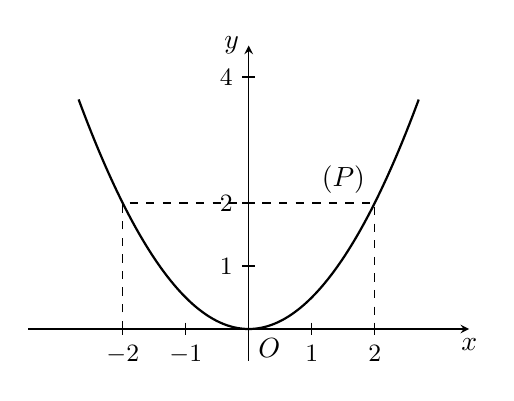
\begin{tikzpicture}[>=stealth,scale=0.8]
			\draw[->] (-3.5,0) -- (3.5,0) node[below] {$x$};
			\draw[->] (0,-0.5) -- (0,4.5) node[left] {$y$};
			\draw (0,0) node[below right] {$O$};
			\foreach \x in {-2,-1,1,2}
				\draw (\x,0.1) -- (\x,-0.1) node[below] {\small $\x$};
			\foreach \y in {1,2,4}
				\draw (0.1,\y) -- (-0.1,\y) node[left] {\small $\y$};
			\draw[dashed] (-2,0) -- (-2,2) -- (2,2) -- (2,0);
			\draw[thick,smooth,samples=100,domain=-2.7:2.7] plot(\x,{0.5*(\x)^2});
			\node[above left] at (2,2) {$(P)$};
		\end{tikzpicture}
	\end{center}
	\item Gọi điểm cần tìm là $M(x; y)$. Vì điểm $M$ có tung độ gấp đôi hoành độ nên $y = 2x$.\\
	Vì $M \in (P)$ nên ta có phương trình:
	$$\dfrac{1}{2}x^2 = 2x \iff \dfrac{1}{2}x^2 - 2x = 0 \iff x\left(\dfrac{1}{2}x - 2\right) = 0 \iff \left[\begin{aligned} &x = 0 \\ &x = 4. \end{aligned}\right.$$
	Vì điểm $M$ khác gốc tọa độ $O(0; 0)$ nên chọn $x = 4 \implies y = 2 \cdot 4 = 8$.\\
	Vậy tọa độ điểm cần tìm là $M(4; 8)$.
\end{enumerate}
}
\end{bt}

\begin{bt}%[9D6H20-2]
% nguon: Đề tham khảo Tuyển sinh 10 năm học 2026-2027 Sở GD&ĐT TP.HCM - Cụm 4 Đề 1 - Bài 2
Cho phương trình bậc hai $3x^2 - 2x - 2 = 0$.
\begin{enumerate}[a)]
	\item Chứng tỏ phương trình luôn có hai nghiệm phân biệt $x_1, x_2$.
	\item Không giải phương trình, hãy tính giá trị của biểu thức:
	$$A = x_1^3 + x_2^3 - 3x_1^2 x_2 - 3x_1 x_2^2.$$
\end{enumerate}
\loigiai{
\begin{enumerate}[a)]
	\item Phương trình $3x^2 - 2x - 2 = 0$ có các hệ số $a = 3$, $b = -2$, $c = -2$.\\
	Biệt thức:
	$$\Delta = b^2 - 4ac = (-2)^2 - 4 \cdot 3 \cdot (-2) = 4 + 24 = 28 > 0.$$
	Vì $\Delta > 0$ nên phương trình luôn có hai nghiệm phân biệt $x_1, x_2$.
	\item Theo định lí Vi-ét, ta có:
	$$\left\{\begin{aligned} &x_1 + x_2 = \dfrac{2}{3} \\ &x_1 x_2 = -\dfrac{2}{3}. \end{aligned}\right.$$
	Ta có:
	$$x_1^2 + x_2^2 = (x_1 + x_2)^2 - 2x_1 x_2 = \left(\dfrac{2}{3}\right)^2 - 2 \cdot \left(-\dfrac{2}{3}\right) = \dfrac{4}{9} + \dfrac{4}{3} = \dfrac{16}{9}.$$
	Biến đổi biểu thức $A$:
	\begin{align*}
		A &= x_1^3 + x_2^3 - 3x_1 x_2(x_1 + x_2) \\
		&= (x_1 + x_2)(x_1^2 - x_1 x_2 + x_2^2) - 3x_1 x_2(x_1 + x_2).
	\end{align*}
	Thay các giá trị của Vi-ét vào, ta được:
	$$A = \dfrac{2}{3} \cdot \left[\dfrac{16}{9} - \left(-\dfrac{2}{3}\right)\right] - 3 \cdot \left(-\dfrac{2}{3}\right) \cdot \dfrac{2}{3} = \dfrac{2}{3} \cdot \dfrac{22}{9} + \dfrac{4}{3} = \dfrac{44}{27} + \dfrac{36}{27} = \dfrac{80}{27}.$$
	Vậy $A = \dfrac{80}{27}$.
\end{enumerate}
}
\end{bt}

\begin{bt}%[9D8H26-3]
% nguon: Đề tham khảo Tuyển sinh 10 năm học 2026-2027 Sở GD&ĐT TP.HCM - Cụm 4 Đề 1 - Bài 3
Có $6$ tấm bìa giống nhau được đánh số từ $1$ đến $6$ (trên mỗi tấm bìa ghi đúng một chữ số). Chọn ngẫu nhiên đồng thời $4$ tấm bìa, xem số ghi trên các tấm bìa rồi sắp xếp chúng theo thứ tự từ nhỏ đến lớn để tạo thành một số có bốn chữ số dạng $\overline{abcd}$ (với $a < b < c < d$). Tính xác suất để số thu được có chữ số cuối lớn hơn chữ số đầu đúng $3$ đơn vị.
\loigiai{
Không gian mẫu là số cách chọn ngẫu nhiên đồng thời $4$ tấm bìa từ $6$ tấm bìa. Vì mỗi cách chọn $4$ số phân biệt luôn được sắp xếp theo thứ tự tăng dần $a < b < c < d$ tạo thành duy nhất một số có bốn chữ số nên số phần tử của không gian mẫu là:
$$n(\Omega) = \dfrac{6 \cdot 5 \cdot 4 \cdot 3}{4 \cdot 3 \cdot 2 \cdot 1} = 15.$$
Các kết quả có thể xảy ra trong không gian mẫu là:
$$\Omega = \{1234; 1235; 1236; 1245; 1246; 1256; 1345; 1346; 1356; 1456; 2345; 2346; 2356; 2456; 3456\}.$$
Gọi $A$ là biến cố: ``Số thu được có chữ số cuối lớn hơn chữ số đầu đúng $3$ đơn vị'', tức là $d - a = 3$ hay $d = a + 3$.\\
Vì $a < b < c < d$ nên các trường hợp thuận lợi cho biến cố $A$ là:
\begin{itemize}
	\item Nếu $a = 1 \implies d = 4$, hai chữ số $b, c$ phải thuộc $\{2; 3\}$ nên có $1$ số là $1234$.
	\item Nếu $a = 2 \implies d = 5$, hai chữ số $b, c$ phải thuộc $\{3; 4\}$ nên có $1$ số là $2345$.
	\item Nếu $a = 3 \implies d = 6$, hai chữ số $b, c$ phải thuộc $\{4; 5\}$ nên có $1$ số là $3456$.
\end{itemize}
Do đó biến cố $A$ có $3$ kết quả thuận lợi: $n(A) = 3$.\\
Xác suất của biến cố $A$ là:
$$P(A) = \dfrac{n(A)}{n(\Omega)} = \dfrac{3}{15} = \dfrac{1}{5}.$$
}
\end{bt}

\begin{bt}%[9D6V21-3]
% nguon: Đề tham khảo Tuyển sinh 10 năm học 2026-2027 Sở GD&ĐT TP.HCM - Cụm 4 Đề 1 - Bài 4
Bác An sở hữu một mảnh đất hình chữ nhật có chiều rộng $x$ mét và chiều dài $y$ mét ($x > 2, y > 0$). Bác chia mảnh đất thành hai khu vực: một hồ nuôi cá hình chữ nhật và một khu trồng cây ăn quả hình vuông. Phần đường đi xung quanh hồ cá và các lối đi qua các đỉnh của hình vuông đất trồng cây đều có bề rộng bằng $1\text{ m}$. Bác An thiết kế sao cho diện tích hồ nuôi cá bằng $4$ lần diện tích khu đất trồng cây. Toàn bộ phần đất còn lại được lát gạch để đi lại.
\begin{enumerate}[a)]
	\item Viết biểu thức tính diện tích phần đất lát gạch $S$ theo $x$ và $y$.
	\item Cho biết diện tích phần đất dành để lát gạch là $50\text{ m}^2$. Hãy tính chiều dài $y$ của khu đất.
\end{enumerate}
\loigiai{
\begin{enumerate}[a)]
	\item Vì lối đi hai bên mép đất đều rộng $1\text{ m}$ nên đường chéo của khu đất hình vuông trồng cây ăn quả là:
	$$d = x - 1 - 1 = x - 2\text{ (m)}.$$
	Diện tích của khu đất hình vuông trồng cây tính theo độ dài đường chéo là:
	$$S_{\text{cây}} = \dfrac{d^2}{2} = \dfrac{(x - 2)^2}{2}\text{ (m}^2\text{)}.$$
	Diện tích của hồ cá gấp $4$ lần diện tích khu đất trồng cây nên:
	$$S_{\text{cá}} = 4 \cdot \dfrac{(x - 2)^2}{2} = 2(x - 2)^2\text{ (m}^2\text{)}.$$
	Diện tích toàn bộ mảnh đất là: $S_{\text{tổng}} = xy\text{ (m}^2\text{)}$.\\
	Biểu thức tính diện tích phần đất dùng để lát gạch là:
	$$S = S_{\text{tổng}} - S_{\text{cá}} - S_{\text{cây}} = xy - 2(x - 2)^2 - \dfrac{(x - 2)^2}{2} = xy - \dfrac{5(x - 2)^2}{2}\text{ (m}^2\text{)}.$$
	\item Chiều rộng của hồ cá hình chữ nhật là $x - 1 - 1 = x - 2\text{ (m)}$.\\
	Chiều dài của hồ cá là $y - 3 - (x - 2) = y - x - 1\text{ (m)}$.\\
	Diện tích hồ cá là:
	$$S_{\text{cá}} = (x - 2)(y - x - 1)\text{ (m}^2\text{)}.$$
	Theo câu a, $S_{\text{cá}} = 2(x - 2)^2$, do đó:
	$$(x - 2)(y - x - 1) = 2(x - 2)^2 \iff (x - 2)[(y - x - 1) - 2(x - 2)] = 0 \iff (x - 2)(y - 3x + 3) = 0.$$
	Vì $x > 2$ nên $x - 2 \neq 0$, suy ra $y - 3x + 3 = 0 \implies y = 3x - 3$.\\
	Theo đề bài, diện tích phần lát gạch là $50\text{ m}^2$, ta có phương trình:
	$$xy - \dfrac{5(x - 2)^2}{2} = 50.$$
	Thay $y = 3x - 3$ vào phương trình, ta được:
	\begin{align*}
		x(3x - 3) - \dfrac{5(x - 2)^2}{2} &= 50 \\
		\iff 3x^2 - 3x - \dfrac{5(x^2 - 4x + 4)}{2} &= 50 \\
		\iff 6x^2 - 6x - 5x^2 + 20x - 20 &= 100 \\
		\iff x^2 + 14x - 120 &= 0.
	\end{align*}
	Giải phương trình bậc hai, ta được $x_1 = 6$ (nhận vì $x > 2$) và $x_2 = -20$ (loại).\\
	Với $x = 6$, ta có chiều dài khu đất là:
	$$y = 3 \cdot 6 - 3 = 15\text{ (m)}.$$
	Vậy chiều dài của khu đất là $15\text{ m}$.
\end{enumerate}
}
\end{bt}

\begin{bt}%[9H0V31-3]
% nguon: Đề tham khảo Tuyển sinh 10 năm học 2026-2027 Sở GD&ĐT TP.HCM - Cụm 4 Đề 1 - Bài 5
Một hồ cá có hình dạng là một phần của hình cầu tâm $O$. Người ta đo được đường kính của miệng hồ hình tròn là $AB = 60\text{ cm}$. Khoảng cách từ miệng hồ đến vị trí sâu nhất $T$ ở đáy hồ là $IT = 90\text{ cm}$ (với $I$ là tâm của miệng hồ, $O, I, T$ thẳng hàng).
\begin{enumerate}[a)]
	\item Tính bán kính $R$ của mặt cầu tạo nên hồ cá.
	\item Người ta rót nước vào hồ sao cho mặt nước cách miệng hồ $40\text{ cm}$. Tính thể tích nước rót vào (kết quả làm tròn đến chữ số thập phân thứ nhất, theo đơn vị lít). Cho biết thể tích hình cầu bán kính $R$ là $V = \dfrac{4}{3}\pi R^3$ và lấy $\pi \approx 3{,}14$.
\end{enumerate}
\loigiai{
\begin{enumerate}[a)]
	\item Vì $AB = 60\text{ cm}$ là đường kính miệng hồ tròn nên bán kính miệng hồ là $IA = \dfrac{AB}{2} = 30\text{ cm}$.\\
	Vì $T$ là điểm sâu nhất nên $OT = R$ là bán kính của mặt cầu.\\
	Do $IT = 90\text{ cm} > R$ nên điểm $O$ nằm giữa $I$ và $T$, suy ra:
	$$OI = IT - OT = 90 - R\text{ (cm)}.$$
	Tam giác $OIA$ vuông tại $I$ (do trục $OI \perp AB$), áp dụng định lí Pythagore:
	\begin{align*}
		OA^2 &= OI^2 + IA^2 \\
		\iff R^2 &= (90 - R)^2 + 30^2 \\
		\iff R^2 &= 8100 - 180R + R^2 + 900 \\
		\iff 180R &= 9000 \implies R = 50\text{ (cm)}.
	\end{align*}
	Vậy bán kính của mặt cầu tạo nên hồ cá là $R = 50\text{ cm}$.
	\item Khoảng cách từ mặt nước đến điểm sâu nhất $T$ của hồ là:
	$$h = IT - 40 = 90 - 40 = 50\text{ (cm)}.$$
	Vì $h = R = 50\text{ cm}$ nên mặt nước đi qua đúng tâm $O$ của mặt cầu.\\
	Do đó khối nước trong hồ tạo thành một nửa hình cầu bán kính $R = 50\text{ cm}$.\\
	Thể tích nước rót vào hồ là:
	$$V_{\text{nước}} = \dfrac{1}{2} \cdot \dfrac{4}{3}\pi R^3 = \dfrac{2}{3}\pi \cdot 50^3 = \dfrac{250\,000\pi}{3}\text{ (cm}^3\text{)}.$$
	Đổi ra đơn vị lít ($1\text{ lít} = 1\,000\text{ cm}^3$):
	$$V_{\text{nước}} = \dfrac{250\pi}{3} \approx \dfrac{250 \cdot 3{,}14159}{3} \approx 261{,}8\text{ (lít)}.$$
	Vậy thể tích nước rót vào hồ xấp xỉ $261{,}8$ lít.
\end{enumerate}
}
\end{bt}

\begin{bt}%[9D1H3-4]
% nguon: Đề tham khảo Tuyển sinh 10 năm học 2026-2027 Sở GD&ĐT TP.HCM - Cụm 4 Đề 1 - Bài 6
Một nhà máy sản xuất nhiên liệu sinh học bằng cách pha trộn hai nguyên liệu là chất A và chất B với nhau. Hiện tại trong kho có $135$ lít chất A và $615$ lít chất B. Để tạo ra nhiên liệu loại I thì tỉ lệ thể tích chất A và chất B là $1 : 9$. Để tạo ra nhiên liệu loại II thì tỉ lệ thể tích chất A và chất B là $1 : 3$. Hỏi nếu sử dụng hết toàn bộ chất A và chất B trong kho thì có thể sản xuất được bao nhiêu lít nhiên liệu loại I và bao nhiêu lít nhiên liệu loại II?
\loigiai{
Gọi $x$ (lít) là số lít nhiên liệu loại I và $y$ (lít) là số lít nhiên liệu loại II sản xuất được ($x, y > 0$).\\
Vì nhiên liệu loại I pha theo tỉ lệ $1 : 9$ (gồm $1 + 9 = 10$ phần) nên trong $x$ lít nhiên liệu loại I có:
\begin{itemize}
	\item $\dfrac{1}{10}x$ lít chất A;
	\item $\dfrac{9}{10}x$ lít chất B.
\end{itemize}
Vì nhiên liệu loại II pha theo tỉ lệ $1 : 3$ (gồm $1 + 3 = 4$ phần) nên trong $y$ lít nhiên liệu loại II có:
\begin{itemize}
	\item $\dfrac{1}{4}y$ lít chất A;
	\item $\dfrac{3}{4}y$ lít chất B.
\end{itemize}
Vì sử dụng hết $135$ lít chất A nên ta có phương trình:
$$\dfrac{1}{10}x + \dfrac{1}{4}y = 135\text{ (1)}.$$
Vì sử dụng hết $615$ lít chất B nên ta có phương trình:
$$\dfrac{9}{10}x + \dfrac{3}{4}y = 615\text{ (2)}.$$
Từ (1) và (2) ta có hệ phương trình bậc nhất hai ẩn:
$$\left\{\begin{aligned} &\dfrac{1}{10}x + \dfrac{1}{4}y = 135 \\ &\dfrac{9}{10}x + \dfrac{3}{4}y = 615 \end{aligned}\right. \iff \left\{\begin{aligned} &2x + 5y = 2700 \\ &18x + 15y = 12300 \end{aligned}\right. \iff \left\{\begin{aligned} &6x + 15y = 8100 \\ &18x + 15y = 12300 \end{aligned}\right. \iff \left\{\begin{aligned} &12x = 4200 \\ &2x + 5y = 2700 \end{aligned}\right. \iff \left\{\begin{aligned} &x = 350 \\ &y = 400. \end{aligned}\right.$$
Cả hai giá trị đều thỏa mãn điều kiện bài toán.\\
Vậy nhà máy có thể sản xuất được $350$ lít nhiên liệu loại I và $400$ lít nhiên liệu loại II.
}
\end{bt}

\begin{bt}%[9H9C29-3]
% nguon: Đề tham khảo Tuyển sinh 10 năm học 2026-2027 Sở GD&ĐT TP.HCM - Cụm 4 Đề 1 - Bài 7
Cho đường tròn $(O)$ có $AB$ là một dây cung không đi qua tâm. Gọi $H$ là trung điểm của đoạn thẳng $AB$. Tiếp tuyến tại $A$ của đường tròn $(O)$ cắt tia $OH$ tại điểm $K$.
\begin{enumerate}[a)]
	\item Chứng minh $\widehat{KBO} = 90^\circ$ và tứ giác $KAOB$ là tứ giác nội tiếp.
	\item Kẻ đường kính $AC$ của đường tròn $(O)$. Chứng minh $OH \cdot OK = OC^2$, từ đó suy ra $\widehat{OCH} = \widehat{OKC}$.
	\item Tiếp tuyến tại $C$ của đường tròn $(O)$ cắt tia $AB$ tại điểm $E$. Gọi $I$ là giao điểm của $OE$ và $KC$. Tính bán kính đường tròn ngoại tiếp tứ giác $KHIE$ biết $\widehat{KAB} = 70^\circ$ và $HI = 6\text{ cm}$ (kết quả làm tròn đến chữ số thập phân thứ hai).
\end{enumerate}
\loigiai{
\begin{center}
	\begin{tikzpicture}[scale=0.9,>=stealth]
		\coordinate (O) at (0,0);
		\def\R{2.8}
		\draw[thick] (O) circle (\R);
		\coordinate (A) at ({-2.8*cos(40)},{2.8*sin(40)});
		\coordinate (C) at ($(O)!-1!(A)$);
		\coordinate (B) at ({-2.8*cos(40)},{-2.8*sin(40)});
		\coordinate (H) at ($(A)!0.5!(B)$);
		\coordinate (K) at ({-2.8/cos(40)},0);
		\coordinate (E) at ({-2.8*cos(40)},{-2.8*(1+cos(40)*cos(40))/sin(40)});
		\coordinate (I) at (intersection of O--E and K--C);

		\draw[thick] (A) -- (C);
		\draw[thick] (A) -- (B) -- (E);
		\draw[thick] (K) -- (A);
		\draw[thick] (K) -- (B);
		\draw[thick] (K) -- (O);
		\draw[thick] (K) -- (C);
		\draw[thick] (O) -- (E);
		\draw[thick] (C) -- (E);
		\draw[dashed] (H) -- (I);

		\fill (O) circle (1.5pt) node[above right] {$O$};
		\fill (A) circle (1.5pt) node[above left] {$A$};
		\fill (B) circle (1.5pt) node[below left] {$B$};
		\fill (C) circle (1.5pt) node[below right] {$C$};
		\fill (H) circle (1.5pt) node[above left] {$H$};
		\fill (K) circle (1.5pt) node[left] {$K$};
		\fill (E) circle (1.5pt) node[below] {$E$};
		\fill (I) circle (1.5pt) node[above] {$I$};
	\end{tikzpicture}
\end{center}
\begin{enumerate}[a)]
	\item Tam giác $OAB$ cân tại $O$ ($OA = OB = R$) có $H$ là trung điểm dây cung $AB$ nên $OH$ đồng thời là đường cao và đường phân giác của góc $\widehat{AOB}$.\\
	Suy ra $OH \perp AB$ và $\widehat{AOK} = \widehat{BOK}$.\\
	Xét $\Delta KAO$ và $\Delta KBO$ có:
	\begin{itemize}
		\item $OA = OB = R$;
		\item Góc $\widehat{AOK} = \widehat{BOK}$;
		\item $OK$ là cạnh chung.
	\end{itemize}
	Do đó $\Delta KAO = \Delta KBO$ (c-g-c), suy ra $\widehat{KBO} = \widehat{KAO} = 90^\circ$ (do $KA$ là tiếp tuyến tại $A$).\\
	Xét tứ giác $KAOB$ có $\widehat{KAO} + \widehat{KBO} = 90^\circ + 90^\circ = 180^\circ$, suy ra $KAOB$ là tứ giác nội tiếp đường tròn đường kính $OK$.
	\item Tam giác $KAO$ vuông tại $A$ có $AH$ là đường cao ($AH \perp OK$ tại $H$), áp dụng hệ thức lượng ta có:
	$$OA^2 = OH \cdot OK.$$
	Vì $OA = OC = R$ nên $OC^2 = OH \cdot OK \implies \dfrac{OH}{OC} = \dfrac{OC}{OK}$.\\
	Xét $\Delta OHC$ và $\Delta OCK$ có:
	\begin{itemize}
		\item Góc $\widehat{COK}$ chung;
		\item $\dfrac{OH}{OC} = \dfrac{OC}{OK}$.
	\end{itemize}
	Do đó $\Delta OHC \backsim \Delta OCK$ (c-g-c), suy ra $\widehat{OCH} = \widehat{OKC}$.
	\item Vì $CE$ là tiếp tuyến của $(O)$ nên $\widehat{OCE} = 90^\circ$.\\
	Tam giác $OCE$ vuông tại $C$ và tam giác $OHE$ vuông tại $H$ đều nội tiếp đường tròn đường kính $OE$, suy ra tứ giác $OHEC$ nội tiếp đường tròn đường kính $OE$.\\
	Do đó $\widehat{OEH} = \widehat{OCH}$ (hai góc nội tiếp cùng chắn cung $OH$).\\
	Theo câu b, $\widehat{OCH} = \widehat{OKC}$ nên $\widehat{OEH} = \widehat{OKI}$.\\
	Xét $\Delta OIK$ và $\Delta OHE$ có:
	\begin{itemize}
		\item Góc $\widehat{KOE}$ chung;
		\item $\widehat{OKI} = \widehat{OEH}$.
	\end{itemize}
	Suy ra $\Delta OIK \backsim \Delta OHE$ (g-g) $\implies \widehat{OIK} = \widehat{OHE} = 90^\circ \implies KC \perp OE$ tại $I$.\\
	Xét tứ giác $KHIE$ có $\widehat{KIE} = 90^\circ$ và $\widehat{KHE} = 90^\circ$, do đó $K, H, I, E$ cùng thuộc đường tròn đường kính $KE$.\\
	Bán kính đường tròn ngoại tiếp tứ giác $KHIE$ là $r = \dfrac{KE}{2}$.\\
	Ta có $\widehat{KAB} = \widehat{AOH} = 70^\circ$ (cùng phụ góc $\widehat{OAH}$). Trong tam giác vuông $OAH$:
	$$AH = R \sin 70^\circ, \quad OH = R \cos 70^\circ.$$
	Kẻ $CD \perp OH$ tại $D$. Ta có $\widehat{COD} = \widehat{AOH} = 70^\circ$ (đối đỉnh).\\
	Trong tam giác vuông $OCD$: $OD = R \cos 70^\circ$, $CD = R \sin 70^\circ$.\\
	Suy ra $HD = HO + OD = 2R \cos 70^\circ$.\\
	Trong tam giác vuông $HCD$:
	$$HC = \sqrt{CD^2 + HD^2} = R\sqrt{\sin^2 70^\circ + 4\cos^2 70^\circ}.$$
	Hai tam giác $\Delta AHC$ và $\Delta AOE$ đồng dạng (g-g) vì có góc $\widehat{A}$ chung và $\widehat{ACH} = \widehat{AEO}$, suy ra:
	$$OE = \dfrac{HC \cdot AO}{AH} = \dfrac{R\sqrt{\sin^2 70^\circ + 4\cos^2 70^\circ}}{\sin 70^\circ}.$$
	Hai tam giác $\Delta OIH$ và $\Delta OKE$ đồng dạng (g-g), suy ra:
	$$\dfrac{HI}{KE} = \dfrac{OH}{OE} \implies KE = HI \cdot \dfrac{OE}{OH}.$$
	Do đó bán kính đường tròn ngoại tiếp tứ giác $KHIE$ là:
	$$r = \dfrac{KE}{2} = \dfrac{HI}{2} \cdot \dfrac{OE}{OH} = \dfrac{6}{2} \cdot \dfrac{\sqrt{\sin^2 70^\circ + 4\cos^2 70^\circ}}{\sin 70^\circ \cdot \cos 70^\circ} \approx 3 \cdot \dfrac{1{,}1623}{0{,}9397 \cdot 0{,}3420} \approx 10{,}85\text{ (cm)}.$$
	Vậy bán kính cần tìm là $10{,}85\text{ cm}$.
\end{enumerate}
}
\end{bt}
